\documentclass[11pt,aps,preprint,nofootinbib,superscriptaddress,tightenlines]{revtex4-2}
\usepackage{amsmath,amssymb,bm,mathtools,graphicx}
\usepackage{xcolor}
\definecolor{darkblue}{RGB}{0,0,160}
\usepackage[colorlinks=true,linkcolor=darkblue,citecolor=darkblue,urlcolor=darkblue]{hyperref}

\def\st{\begin{equation}}
\def\stp{\end{equation}}
\def\Eq#1{eq.~(\ref{#1})}
\def\Sect#1{Sect.~\ref{#1}}
\def\Fig#1{Fig.~\ref{#1}}
\usepackage{dsfont}
\newcommand{\one}{\mathds{1}}
\newcommand{\pf}{\bm{\mathsf p}}
\DeclareMathOperator{\tr}{tr}
\newcommand{\avg}[1]{\langle #1\rangle}
\let\oldparagraph\paragraph
\renewcommand{\paragraph}{\par\bigskip\oldparagraph}

\begin{document}

\title{A stochastic viscous step in the particle representation: plan}
\author{D.~Teaney}
\affiliation{Department of Physics and Astronomy, Stony Brook University,
Stony Brook, New York 11794, USA}
\date{\today}

\begin{abstract}
The deterministic viscous step in the particle representation
(\texttt{changerep.tex}) holds each particle's energy fixed and moves momentum
between particles so that the total particle entropy increases.  Here we plan
its stochastic version: random momentum transfers, accepted or rejected with
the exact change of the particle entropy.  The noise is fixed by the
fluctuation--dissipation theorem through the quadratic form of the bond
dissipative function, written as a sum of local pieces, one per bond and one
per particle.  This note records the plan and the questions to settle before
coding.
\end{abstract}

\maketitle

%=============================================================================
\section{The state and the entropy}
\label{sec:state}

During the viscous step the positions are fixed.  Each particle has a fixed
volume $V_a=s_a/S_a$ and a fixed energy, which with the gradient correction is
$e_a'=e_a-g_a$ (\texttt{changerep.tex}, Appendix~A).  The momenta $\bm m_a$ move.
The stochastic step maximizes the particle entropy subject to constraints on
each particle's energy and on the energy of its long-wavelength gradient.
During a sweep we therefore hold both $e_a'$ and the gradient energy $g_a$ fixed,
so each particle's energy $e_a=e_a'+g_a$ is fixed, and the total particle entropy
is
\st
\mathbb S[\bm m]=\sum_aS_a\big(e_a,\ \bm m_a\big),\qquad
\frac{\partial\mathbb S}{\partial\bm m_a}=-\beta_a ,
\label{Sbb}
\stp
local in each particle.  The gradient energy is updated only at the end, in the
back map $s_a'=S_a(e_a'+g_a',\bm m_a')$ of \texttt{changerep.tex}, as in the
deterministic step.

The stochastic step should leave the distribution $e^{\mathbb S}$ at fixed
energies and total momentum invariant.  In equilibrium every particle-scale
momentum mode then carries its thermal share, $\avg{|\bm m_{\bm k}|^2}\propto wTV$,
at all $k$.  This is the point of the change of representation: with the
smoothed $\beta$ the short-wavelength modes are damped by $R^2$ while their
noise is not, and they run away.

%=============================================================================
\section{A stress proposal}
\label{sec:stress}

The stochastic step is a Metropolis update of the momenta.  A momentum change
$\delta\bm m$, conserving the total momentum, is drawn from a symmetric Gaussian
with covariance $\Sigma$ and accepted with a probability that depends on the
change of the particle entropy $\Delta\mathbb S$.  For small proposals the mean
change is
\st
\avg{\Delta\bm m}\simeq\frac12\,\Sigma\,\frac{\partial\mathbb S}{\partial\bm m}=-\frac12\,\Sigma\,\beta .
\stp
The deterministic step is $\Delta\bm m=-\Delta t\,\mathcal K\beta$, with $\mathcal K$ the
quadratic form of the dissipative function, so the two agree for
\st
\Sigma=2\Delta t\,\mathcal K ,
\stp
the fluctuation--dissipation theorem.  The dissipative function is a sum of
local pieces, $K=\sum_aK_a$, each depending only on the star of $a$, so the noise
can be built one particle at a time.  We build it from a random stress, start
at rest, and check its mean traction.

\paragraph{The move.}  For particle $a$:
\begin{enumerate}
\item \emph{Draw a random stress} $\xi_a^{ij}$, symmetric, with zero mean and
  variance
  \st
  \avg{\xi_a^{ij}\xi_a^{lm}}=\frac{2\Delta t\,(T_{\rm rel})_a}{V_a}\,\kappa_a^{ijlm},
  \label{xivar}
  \stp
  where $(T_{\rm rel})_a$ is the rest-frame temperature of particle $a$.  Our
  normal temperature is $T_a=\partial H/\partial s_a=(T_{\rm rel})_a/\gamma_a$, with
  $\beta_a=\bm v_a/T_a$; the rest-frame temperature appears only with the viscous
  coefficients, $T_{\rm rel}\kappa$, $T_{\rm rel}\eta$, $T_{\rm rel}\zeta$, which fix the
  noise.  At rest the two coincide.  Further, $\kappa^{ijlm}$ is the viscous tensor at rest,
  \st
  \kappa^{ijlm}=\eta\Big(\delta^{il}\delta^{jm}+\delta^{im}\delta^{jl}-\frac2d\,\delta^{ij}\delta^{lm}\Big)+\zeta\,\delta^{ij}\delta^{lm}.
  \stp
\item \emph{Distribute it across the star.}  Each face of $a$ carries the
  traction
  \st
  \pf_{ab}=\xi_a\bm A_{ab},\qquad \bm A_{ab}=V_a\,w_{ab}\,\bm r_{ab},
  \label{tstress}
  \stp
  with $\bm A_{ab}$ the face of \texttt{bond\_dissipation.tex}.  Particle $b$
  receives $\pf_{ab}$ and $a$ gives up their sum:
  \st
  \delta\bm m_b=\pf_{ab},\qquad \delta\bm m_a=-\sum_{b\neq a}\pf_{ab}.
  \stp
  Momentum is conserved.  By the closure of the faces the virial of the
  tractions is the stress itself,
  \st
  \sum_{b\neq a}\pf_{ab}\,\bm r_{ab}^T=V_a\,\xi_a ,
  \stp
  which is symmetric, so the faces exert no net torque.  This is the
  angular-momentum constraint.
\item \emph{Ask the star.}  Accept or reject the whole proposal by the
  consensus of its bonds, described next.  On rejection the star is left
  untouched.
\end{enumerate}
Each particle in turn does the same, so particle $b$, with its own stress
$\xi_b$ of variance $\kappa_b$, gives the traction $\pf_{ba}$ to $a$.

\paragraph{The consensus.}  The proposal changes the entropy of $a$ and of every
member of its star,
\st
\Delta\mathbb S=\Delta S_a+\sum_{b\neq a}\Delta S_b .
\label{dStot}
\stp
We write this as a sum over the bonds,
\st
\Delta\mathbb S=\sum_{b\neq a}\Delta S_{ab} ,
\label{dSbonds}
\stp
with one term per bond, specified below.  A single vote would accept the
proposal with probability $\min(1,e^{\Delta\mathbb S})$.  Instead each bond votes,
accepting with probability $\min(1,e^{\Delta S_{ab}})$, and the proposal is kept
only if every bond accepts:
\st
P(\xi_a)=\prod_{b\neq a}\min\big(1,e^{\Delta S_{ab}}\big).
\label{Pfact}
\stp
If any bond rejects, the whole proposal is rejected.  This is a factorized
Metropolis filter.  Like the single vote, it satisfies detailed balance with
respect to $e^{\mathbb S}$, provided
\begin{enumerate}
\item the bond terms add up to $\Delta\mathbb S$, \Eq{dSbonds};
\item each bond term flips its sign exactly under the reverse move, which
  starts from the new momenta and proposes $-\pf_{ab}$ on every bond.
\end{enumerate}
It rejects more often than the single vote: a bond that loses entropy can
veto the move even when the others gain more.

\paragraph{Partitioning $\Delta S_a$.}  Particle $b$ receives only the traction
$\pf_{ab}$, so $\Delta S_b$ belongs to the bond $ab$.  Particle $a$ gives up the sum
of all its tractions, so $\Delta S_a$ has to be divided among the bonds:
\st
\Delta S_a=\sum_{b\neq a}\delta S_{ab},\qquad
\Delta S_{ab}=\delta S_{ab}+\Delta S_b .
\label{dSab}
\stp
Condition 1 then holds for any partition; condition 2 requires each
$\delta S_{ab}$ to flip its sign under the reverse move.  (Counting $\Delta S_a$ in
full on every bond would violate condition 1.)  We take
\st
\delta S_{ab}=\sigma_{ab}+\frac{R_a}{n_{\rm b}} ,
\stp
where $\sigma_{ab}$ is the part of $\Delta S_a$ due to $\pf_{ab}$, $R_a$ is the rest, and
$n_{\rm b}$ is the number of bonds of $a$.

For $\sigma_{ab}$, with $\bm m_a$ and
$\bm m_a'=\bm m_a+\delta\bm m_a$ the momenta of $a$ before and after the move,
\st
\sigma_{ab}=\frac12\Big[S_a(\bm m_a-\pf_{ab})-S_a(\bm m_a)\Big]
-\frac12\Big[S_a(\bm m_a'+\pf_{ab})-S_a(\bm m_a')\Big],
\label{sigmaab}
\stp
at fixed $e_a$, and the rest
\st
R_a=\Delta S_a-\sum_{b\neq a}\sigma_{ab}
\stp
is split evenly.  The reverse move exchanges $\bm m_a$ and $\bm m_a'$ and flips
$\pf_{ab}$, so it flips the sign of each $\sigma_{ab}$ exactly, and of $R_a$:
condition 2 holds.  To leading order $\sigma_{ab}\simeq\beta_a\cdot\pf_{ab}$, $R_a$ is of
third order, and
\st
\Delta S_{ab}\simeq-\big(\beta_b-\beta_a\big)\cdot\pf_{ab} :
\stp
each factor is the entropy produced by the bond itself.  It depends only on the
difference $\beta_b-\beta_a$, so it vanishes for a uniformly moving fluid, as the
dissipation does.

For an entropy quadratic in the momentum the second-order terms
cancel in \Eq{sigmaab}, and
\st
\sigma_{ab}=\beta_a^{\rm mid}\cdot\pf_{ab},\qquad
\Delta S_b=-\beta_b^{\rm mid}\cdot\pf_{ab},
\stp
where $\beta^{\rm mid}$ is evaluated at the midpoint of each particle's move:
$\beta_a^{\rm mid}$ at the average of $\bm m_a$ and $\bm m_a'$, and $\beta_b^{\rm mid}$ at
$\bm m_b+\pf_{ab}/2$.  The bond factor is then
\st
\Delta S_{ab}=-\big(\beta_b^{\rm mid}-\beta_a^{\rm mid}\big)\cdot\pf_{ab} ,
\stp
the entropy produced by the bond, with the midpoint $\beta$ at each end, exact up
to third-order terms, which go into $R_a$.

The simpler even split, $\delta S_{ab}=\Delta S_a/n_{\rm b}$, also satisfies both
conditions, but it
is not invariant under a uniform shift of $\beta$: in a fluid moving with
velocity $\bm v$, $\Delta S_b\simeq-\beta_b\cdot\pf_{ab}$ contains $-(\bm v/T)\cdot\pf_{ab}$,
which is large and of random sign, and the bonds reject even though nothing
dissipates.  In a fluid moving at $v=0.32$, the even split accepts 7\% of the
residual moves in 2D, and \Eq{sigmaab} 47\%, the same as at rest.

\paragraph{The mean traction.}  For a small proposal the entropy change is
linear in the momentum changes, with $\partial S_c/\partial\bm m_c=-\beta_c$:
\st
\Delta\mathbb S=-\sum_{b\neq a}\Delta\beta_{ab}\cdot\pf_{ab}
=-V_a\,\xi_a{:}(\nabla\beta)_a,\qquad
(\nabla\beta)_a=\sum_{b\neq a}w_{ab}\,\Delta\beta_{ab}\,\bm r_{ab}^T ,
\stp
where $(\nabla\beta)_a$ is the fitted gradient of $\beta$ at $a$
(\texttt{bond\_dissipation.tex}, mean-field form) and $\Delta\beta_{ab}=\beta_b-\beta_a$.  The proposal sees $\beta$ only
through $(\nabla\beta)_a$.

\paragraph{Mean of the accepted stress.}  Each factor of \Eq{Pfact} is linear in
the proposal to leading order,
\st
\Delta S_{ab}\simeq g_{ab}{:}\xi_a ,\qquad
\sum_{b\neq a}g_{ab}=\frac{\partial\Delta\mathbb S}{\partial\xi_a}=-V_a(\nabla\beta)_a ,
\stp
and is of order $\sqrt{\Delta t}$.  To the same order the acceptance probability
is
\st
P(\xi_a)\simeq1+\sum_{b\neq a}\min\big(0,\ g_{ab}{:}\xi_a\big).
\stp
The proposal has zero mean, so the mean of the accepted stress is
\st
\avg{\xi_a\,P(\xi_a)}=\sum_{b\neq a}\avg{\xi_a\,\min\big(0,\ x_b\big)},\qquad
x_b=g_{ab}{:}\xi_a .
\stp
Write $C=\avg{\xi_a\xi_a}$ for the covariance \Eq{xivar}.  For a Gaussian $\xi_a$
the part of $\xi_a$ correlated with $x_b$ is $C{:}g_{ab}\,x_b/\avg{x_b^2}$, and the
rest is independent of $x_b$, so
\st
\avg{\xi_a\,\min(0,x_b)}=\frac{C{:}g_{ab}}{\avg{x_b^2}}\,\avg{x_b\min(0,x_b)}
=\frac12\,C{:}g_{ab} ,
\stp
since $x_b\min(0,x_b)$ is $x_b^2$ for half of the Gaussian and zero otherwise.
Summing over the bonds,
\st
\avg{\xi_aP(\xi_a)}=\frac12\,C{:}\frac{\partial\Delta\mathbb S}{\partial\xi_a}
=-\Delta t\,(T_{\rm rel})_a\,\kappa_a{:}(\nabla\beta)_a=\Delta t\,\Pi_a(\nabla\beta) ,
\stp
the viscous stress of the fitted gradient.  A single test on the whole star,
$\min(1,e^{\Delta\mathbb S})$, gives the same mean: the factorization changes
the rejection rate, not the drift.  The mean traction is therefore
\st
\avg{\pf_{ab}}=\Delta t\,\Pi_a(\nabla\beta)\,\bm A_{ab} .
\label{tmean}
\stp
Compare the deterministic traction of the bond form,
\st
\pf_{ab}^{\rm det}=-(2T_{\rm rel}\eta)_a\,V_aw_{ab}\,\mathcal D_{ab}\beta
=\Pi_a(\nabla\beta)\,\bm A_{ab}-(2T_{\rm rel}\eta)_a\,V_aw_{ab}\,\delta_{ab}\beta,
\stp
where $\delta_{ab}\beta=\Delta\beta_{ab}-(\nabla\beta)_a\,\bm r_{ab}$ is the residual of the fit
(\texttt{bond\_dissipation.tex}, resolved plus residual).
\begin{itemize}
\item For a linear field the residual vanishes and \Eq{tmean} is the
  deterministic traction: shear, bulk and rotation all come out right.
\item For a general field \Eq{tmean} is the traction of the \emph{resolved} part
  of $K$ only.  The residual part, which damps the modes the fit cannot see, is
  missing.  Those modes are then neither damped nor excited by the noise.
\end{itemize}
%=============================================================================
\section{The residual move}
\label{sec:resid}

\paragraph{The missing part.}  The dissipative function splits exactly into a
resolved and a residual part, with no cross term
(\texttt{bond\_dissipation.tex}):
\st
K=K_{\rm res}+K_{\rm resid},\qquad
K_{\rm resid}=\sum_a(T_{\rm rel}\eta)_a\sum_{b\neq a}V_aw_{ab}\,|\delta_{ab}\beta|^2 .
\stp
The stress move of \Sect{sec:stress} is the noise of $K_{\rm res}$.  The noise of
$K_{\rm resid}$ is added on top of it, as a second, independent move.  Since there
is no cross term, the covariances add, and so do the mean tractions.

\paragraph{The move.}  For particle $a$:
\begin{enumerate}
\item \emph{Draw a random vector on each bond}, independent from bond to bond,
  with zero mean and variance
  \st
  \avg{\mathfrak p_{ab}\mathfrak p_{ab}^T}=2\Delta t\cdot (2T_{\rm rel}\eta)_a\,V_aw_{ab}\,\one .
  \stp
  In 1D replace $2\eta_a$ by $\kappa_a$.
\item \emph{Remove the part the fit sees.}  The virial of the draws,
  $\sum_{c\neq a}\mathfrak p_{ac}\,\bm r_{ac}^T$, is a stress.  Subtract it,
  distributed through the faces.  The residual traction is
  \st
  \vec p_{ab}=\mathfrak p_{ab}-\frac1{V_a}\Big(\sum_{c\neq a}\mathfrak p_{ac}\,\bm r_{ac}^T\Big)\bm A_{ab} .
  \label{tauab}
  \stp
  Vectors are columns, so the virial is a matrix acting on the face vector
  $\bm A_{ab}$.  In components the second (bond) index of the virial is
  contracted with the face,
  $\vec p^{\,i}_{ab}=\mathfrak p^i_{ab}-V_a^{-1}\sum_c\mathfrak p^i_{ac}\,r^k_{ac}\,A_{ab\,k}$.
  By the closure of the faces, $\sum_{b\neq a}\bm A_{ab}\,\bm r_{ab}^T=V_a\one$,
  its virial vanishes,
  \st
  \sum_{b\neq a}\vec p_{ab}\,\bm r_{ab}^T
  =\sum_{c\neq a}\mathfrak p_{ac}\,\bm r_{ac}^T-\sum_{c\neq a}\mathfrak p_{ac}\,\bm r_{ac}^T=0 ,
  \stp
  so the residual tractions carry no stress and exert no torque.
\item \emph{Kick and ask the bonds.}  Particle $b$ receives $\vec p_{ab}$ and $a$
  gives up their sum.  Accept with the factorized filter \Eq{Pfact}, with the
  bond factors \Eq{dSab}.
\end{enumerate}

\paragraph{The mean traction.}  To leading order the entropy change of the
star is
\st
\Delta\mathbb S=-\sum_{b\neq a}\Delta\beta_{ab}\cdot\vec p_{ab}
=-\sum_{b\neq a}\mathfrak p_{ab}\cdot\delta_{ab}\beta ,
\stp
because the subtracted stress removes $\sum_{c\neq a}\mathfrak p_{ac}\cdot (\nabla\beta)_a\bm r_{ac}$
from the pair term.  The argument of \Sect{sec:stress} gives
\st
\avg{\mathfrak p_{ab}}=-\Delta t\cdot (2T_{\rm rel}\eta)_a\,V_aw_{ab}\,\delta_{ab}\beta .
\stp
The residuals are orthogonal to the bonds,
\st
\sum_{b\neq a}w_{ab}\,\delta_{ab}\beta\,\bm r_{ab}^T=0 ,
\stp
so the mean of the virial of the draws vanishes, and so does the mean of the
subtracted stress.
The mean residual traction is
\st
\avg{\vec p_{ab}}=-\Delta t\cdot (2T_{\rm rel}\eta)_a\,V_aw_{ab}\,\delta_{ab}\beta .
\stp
Added to the mean stress traction \Eq{tmean},
\st
\avg{\pf_{ab}}+\avg{\vec p_{ab}}
=\Delta t\Big[\Pi_a(\nabla\beta)\,\bm A_{ab}-(2T_{\rm rel}\eta)_a\,V_aw_{ab}\,\delta_{ab}\beta\Big]
=\Delta t\,\pf^{\rm det}_{ab} ,
\stp
the deterministic traction of the bond form, on every bond.

\paragraph{One vote or two.}  The two moves could also be drawn together and
accepted by a single vote.  Both are exact.  We take two separate moves:
\begin{itemize}
\item The stress move stays as in \Sect{sec:stress}.
\item Each vote sees less noise, so each is rejected less often.
\item The residual move can be switched off, to check that it is what damps the
  modes the fit cannot see.
\end{itemize}
In 1D there is no rotation, and the residual move is what damps the zone-edge
mode.

\paragraph{A cold residual.}  The residual move need not satisfy detailed
balance.  The modes it acts on are lattice modes, which we want damped but do
not need to fluctuate.  A one-parameter family keeps its mean traction and
reduces its noise.  For $\lambda\geq1$:
\begin{itemize}
\item shrink the proposal covariance by $1/\lambda$;
\item accept with $\min(1,e^{\lambda\Delta S_{ab}})$ in place of
  $\min(1,e^{\Delta S_{ab}})$ in \Eq{Pfact}.
\end{itemize}
By the argument of \Sect{sec:stress}, the mean is multiplied by $\lambda$ through
the acceptance and divided by $\lambda$ through the covariance, so the mean
residual traction is unchanged.  The noise is reduced by $1/\lambda$: the
residual drives the modes toward the temperature $T/\lambda$.
\begin{itemize}
\item $\lambda=1$ is detailed balance.
\item $\lambda\to\infty$ is the deterministic residual step, done directly: the
  residual part of the force of \texttt{changerep.tex}, at fixed $e_a$, with no
  accept/reject.
\end{itemize}
The argument requires the exponent $\lambda\Delta S_{ab}$ to be small.  It is of
order $\sqrt{\lambda\Delta t}$, so the family holds for $\lambda\Delta t\ll1$.

The reduction of the covariance is essential.  Raising the exponent alone, or
accepting only moves with $\Delta S>0$, gives a mean kick of fixed size, of order
$\sqrt{\Delta t}$, along the gradient, independent of the residual itself.
That is a friction of fixed magnitude, not a viscosity, and it does not
converge as $\Delta t\to0$.

\paragraph{The effective temperature.}  A mode of wavenumber $k$ receives noise
from the stress move at temperature $T$ and from the residual move at
temperature $T/\lambda$, and is damped by both.  Its steady state has
\st
\frac{T_{\rm eff}(k)}{T}=\frac{K_{\rm res}(k)+K_{\rm resid}(k)/\lambda}{K_{\rm res}(k)+K_{\rm resid}(k)} .
\label{Teff}
\stp
For a smooth mode $K_{\rm res}\propto k^2$ and $K_{\rm resid}\propto k^4h^2$, so
\st
\frac{T_{\rm eff}(k)}{T}=1-O\big((kh)^2\big) ,
\stp
and the hydrodynamic modes fluctuate at the right temperature.  At the zone
edge the fit sees nothing, $K_{\rm res}=0$, and $T_{\rm eff}=T/\lambda$.  In
between the crossover is smooth.  This is a smooth regulator: the
cutoff-dependent renormalization of the transport coefficients comes from the
thermal modes up to the cutoff, now weighted by \Eq{Teff}.  The counterterm
changes, but it can be computed in the same way.  The total entropy is, to
quadratic order, a constant minus the kinetic energy over $T$, so the steady
state does not heat.

%=============================================================================
\section{The sweep}
\label{sec:sweep}

\paragraph{Independent moves.}  A move of particle $a$ kicks only its star,
the particles within $2h$, and its $\Delta\mathbb S$ involves only those
particles, since $\mathbb S$ is a sum of single-particle entropies at fixed $e_a$
and $V_a$.  Two moves therefore commute exactly when their centres are more than
$4h$ apart.

\paragraph{Checkerboard.}  The cells of the cell list have side at least $2h$.
Color them by their indices modulo 3 in each direction: 9 colors in 2D, 3 in
1D.  Cells of the same color are then at least two cells, i.e.\ $4h$, apart,
and the moves in them are independent.  If the number of cells in a direction
is not a multiple of 3, the periodic wrap breaks the pattern; either choose it
a multiple of 3 or give the leftover column its own color.  One sweep:
\begin{enumerate}
\item Visit the colors in a random order.
\item Within a color, treat every active cell independently (in parallel).
\item Inside a cell, visit its particles in a random order, or pick particles
  at random.  Each particle makes its stress move, using the current momenta.
\end{enumerate}
The residual moves are made in a second, separate sweep of the same form, after
the stress sweep is complete.  The order of the two sweeps can be alternated
from step to step.
Each move satisfies detailed balance on its own, and moves of the same color
act on disjoint sets, so each sweep leaves $e^{\mathbb S}$ stationary, and so
does their composition.  The mean drifts of the two sweeps add to the
deterministic step at leading order in $\Delta t$.  Nothing
is double counted: every accepted move sees the momenta left by the previous
ones.  The random color order makes the sweep reversible on average.

\paragraph{Details.}
\begin{itemize}
\item \emph{Frozen coefficients.}  The variances depend on $(T_{\rm rel})_a$, $w_{ab}$ and the
  fit.  They are computed at the start of the viscous step and held fixed, so
  that each proposal is a fixed symmetric Gaussian and the Metropolis test is
  exact.  Recomputing them from the current momenta would make the proposal
  depend on the state and require a Hastings correction.
\item \emph{Random grid shift.}  Before each sweep the grid of cells is shifted
  by a random vector $\bm u$, uniform within one cell, and the particles are
  re-binned by $\bm x_a+\bm u$ (modulo the box).  Only the partition into cells
  changes; the stars are frozen and do not depend on it.  The cells keep their
  size, so they still tile the box and are at least $2h$ wide.  The re-binning
  is a single pass over the particles.  With fixed positions the shift is not
  needed for correctness; it removes any imprint of the cell boundaries.
\item \emph{Random streams.}  One stream per cell or per particle, not per
  thread, so the results do not depend on the number of threads.
\item \emph{Mean drift.}  Earlier moves shift the momenta of a star by
  zero-mean noise of order $\sqrt{\Delta t}$.  At leading order in $\Delta t$ the
  mean drift is still the deterministic step.
\end{itemize}

\paragraph{Pseudo-code.}  As implemented in \texttt{src/stochastic.jl}
(\texttt{stochastic\_step!}).  The colors along a direction of $n$ cells are
$0,1,2,0,1,2,\dots$ for the first $3\lfloor n/3\rfloor$ cells and $3,4$ for the
one or two leftover cells; the color of a cell is the pair of its two colors.
\begin{verbatim}
stochastic_step!(particles, dt; lambda):
    # frozen for the step (or for the whole run on a frozen lattice)
    for each particle a:
        V[a], e[a]                          # particle volume and energy
        star[a] = bonds b within 2h:  r_ab, w_ab, c_ab
        Trel_a, eta_a, zeta_eff_a              # rest frame
    m[a] = current momenta;  S[a] = S_a(e[a], m[a])
    for kind in (stress, residual)          # order alternates step to step
        if kind == residual and lambda == Inf
            deterministic residual step;  continue
        u = random vector within one cell;  re-bin particles by x + u
        for color in random_permutation(colors)
            parallel for cell in cells_of(color)
                for a in random_permutation(particles_in(cell))
                    move(a, kind)
    write back m[a] and s[a] = S[a]

move(a, kind):                              # random numbers from rngs[a]
    if kind == stress
        xi = random symmetric stress, <xi xi> = 2 dt Trel_a kappa_a / V_a
        delta[b] = xi A_ab,                 A_ab = V_a w_ab r_ab
        lam = 1
    else
        y[b] = random vector, <y y^T> = 2 dt c_ab / lambda
        Y = sum_b y[b] r_ab^T
        delta[b] = y[b] - (Y / V_a) A_ab
        lam = lambda
    delta_a = - sum_b delta[b]
    m'_a = m[a] + delta_a
    dSa  = S_a(e[a], m'_a) - S[a]
    for b:  sigma[b] = (S_a(m[a] - delta[b]) - S_a(m[a]))/2
                     - (S_a(m'_a + delta[b]) - S_a(m'_a))/2
    R    = dSa - sum_b sigma[b]
    logP = sum_b min(0, lam (S_b(e[b], m[b] + delta[b]) - S[b]
                             + sigma[b] + R/n_a))
    if log(uniform) < logP:                 # all or nothing
        m[b] += delta[b] for every bond;  m[a] += delta_a;  update S
\end{verbatim}
A single vote of the star, $\log P=\min(0,\lambda\,\Delta\mathbb S)$, is also
available (\texttt{vote=:star}); it is exact as well and rejects less often.
The even split is \texttt{vote=:even}.

%=============================================================================
\section{Tests on a frozen lattice}
\label{sec:tests}

\paragraph{Setup.}  A lattice of particles with equal particle energies $e_a$
and zero momenta.  Positions, volumes $V_a$ and energies $e_a$ are fixed; only the
viscous step acts.  The conformal equation of state with $\eta/s=0.2$, $\zeta=0$.
\begin{itemize}
\item 1D: $h=0.05$, $h/a=4$, $L=1$ (80 particles), 15 bonds per star.
\item 2D: hexagonal lattice, $h=0.05$, $h/a=2.5$, a box of side $0.6$ (1020
  particles), 88 bonds per star.
\end{itemize}
The entropy per particle is $s_a=500$ (1D) and $346$ (2D), so the thermal
velocities are small, about $0.05$.  The time step is a quarter of the default
viscous half step of \texttt{changerep.tex}.  Scripts:
\texttt{examples/stochastic\_thermalize.jl}, \texttt{examples/stochastic\_smallk.jl}.

\paragraph{The equilibrium value.}  For one particle at fixed $e_a$, $e^{S_a(e_a,\bm m)}$
gives each momentum component the variance $V_awT$ to leading order.  A direct
numerical integral gives $0.993\,V_awT$ at $s_a=500$; the difference is a
relativistic correction.  This is the reference value below.

\paragraph{Detailed balance.}  With $\lambda=1$ the sweep must reproduce it
exactly, for any $\Delta t$.  Starting from a thermal draw, the time-averaged
$\avg{m^2}/(V_awT)$ in 1D is $0.990\pm0.004$ with the bond vote,
$0.991\pm0.003$ with the even split and $0.996\pm0.004$ with the single vote, and
$0.992\pm0.004$ with the grid shift.

\paragraph{The residual damping.}  For a single small mode, one deterministic
residual step reduces the amplitude at exactly the rate
$2K_{\rm resid}(k)/(V_awT)$ predicted by the star (ratio $1.0000$ for every $k$).

\paragraph{Thermalization.}  \Fig{fig:therm1d} and \Fig{fig:therm2d}.  From
zero momenta the spectrum fills in from the zone edge, where the damping is
fastest, and each mode approaches its equilibrium as
$1-e^{-2\Gamma_kt}$, with $\Gamma_k$ the damping rate of the bond form.  The
late-time spectrum is flat for $\lambda=1$ and follows $T_{\rm eff}(k)/T$, \Eq{Teff},
for $\lambda=4$ and $\lambda=\infty$, with no fitted parameter.  In 2D this holds for
both polarizations.  The modes damped mostly by the residual approach their
equilibrium somewhat more slowly than predicted, because of the rejections.

\begin{figure}[t]
\centering
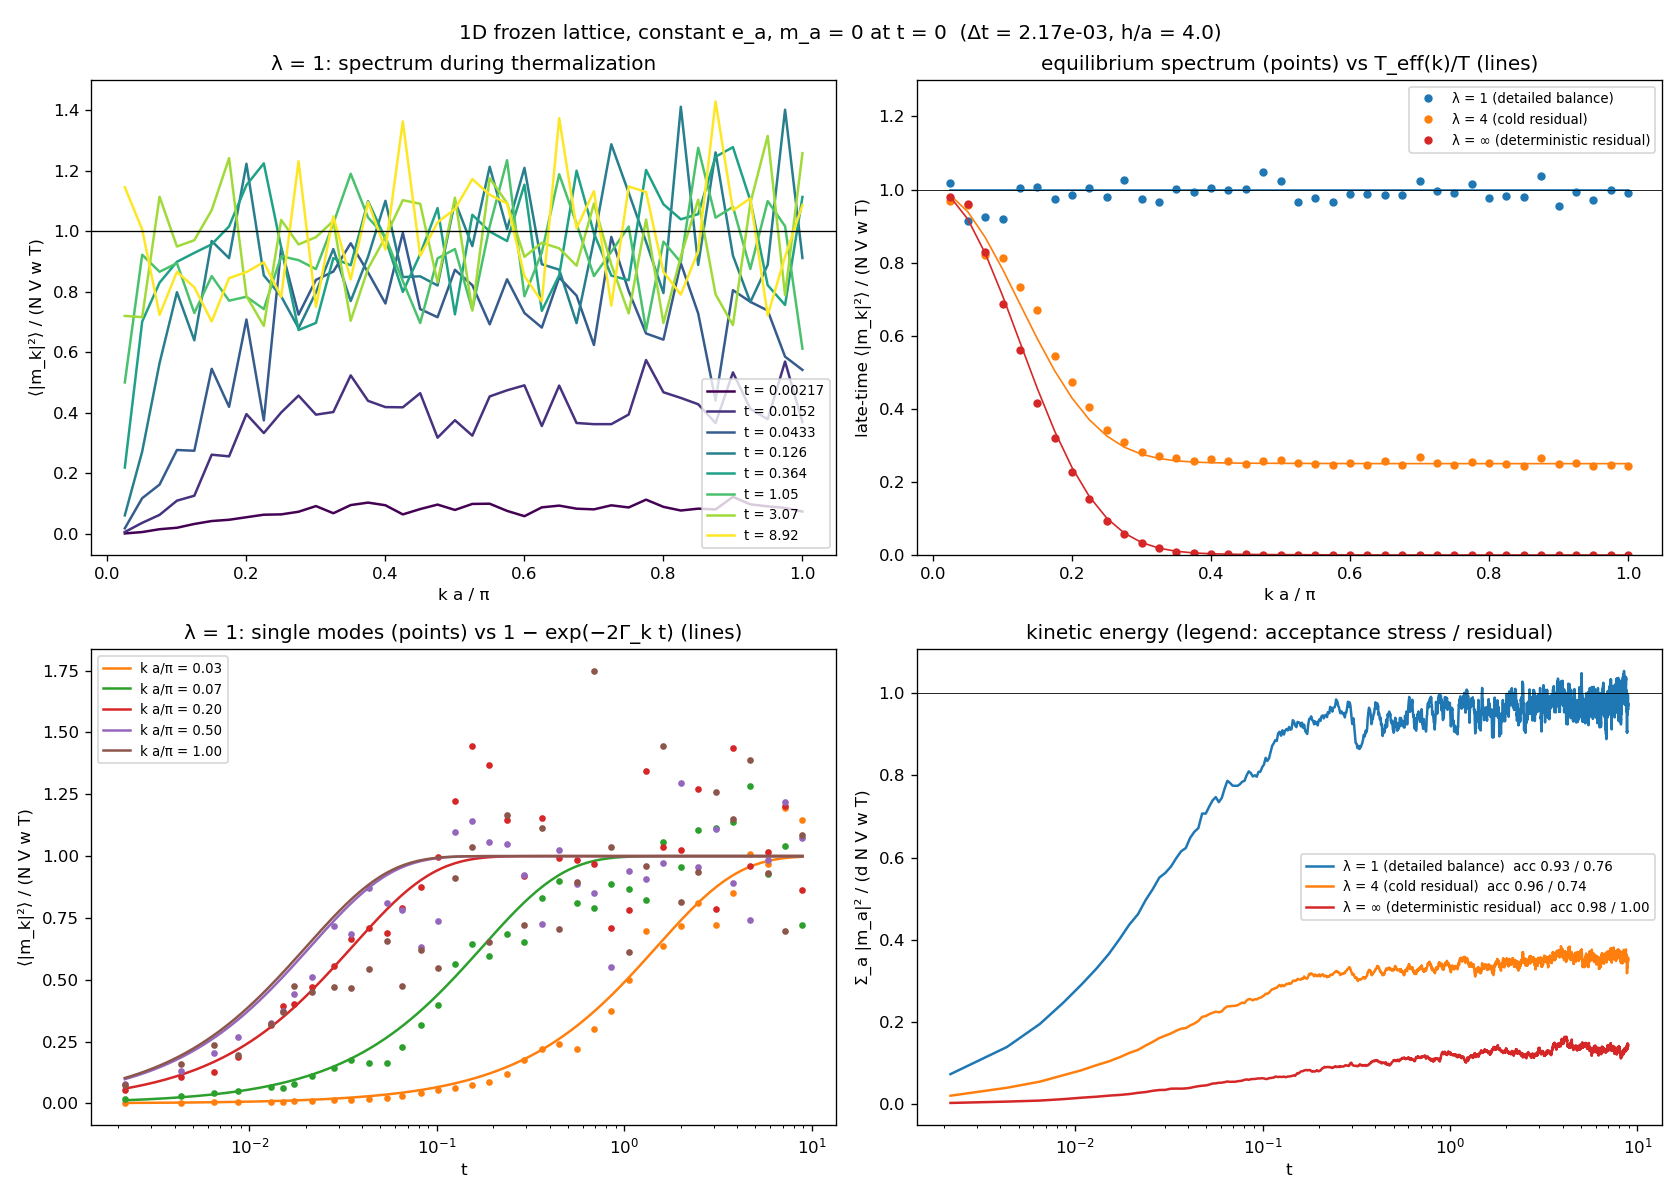
\includegraphics[width=\textwidth]{figs/stochrep_thermalize_1d.png}
\caption{1D frozen lattice, thermalization from zero momenta.  Top left: the
spectrum at several times ($\lambda=1$).  Top right: the late-time spectrum for
$\lambda=1,4,\infty$ (points) and $T_{\rm eff}(k)/T$ (lines).  Bottom left: single modes
(points) and $1-e^{-2\Gamma_kt}$ (lines).  Bottom right: kinetic energy, and
the acceptance of the stress and residual moves.}
\label{fig:therm1d}
\end{figure}

\begin{figure}[t]
\centering
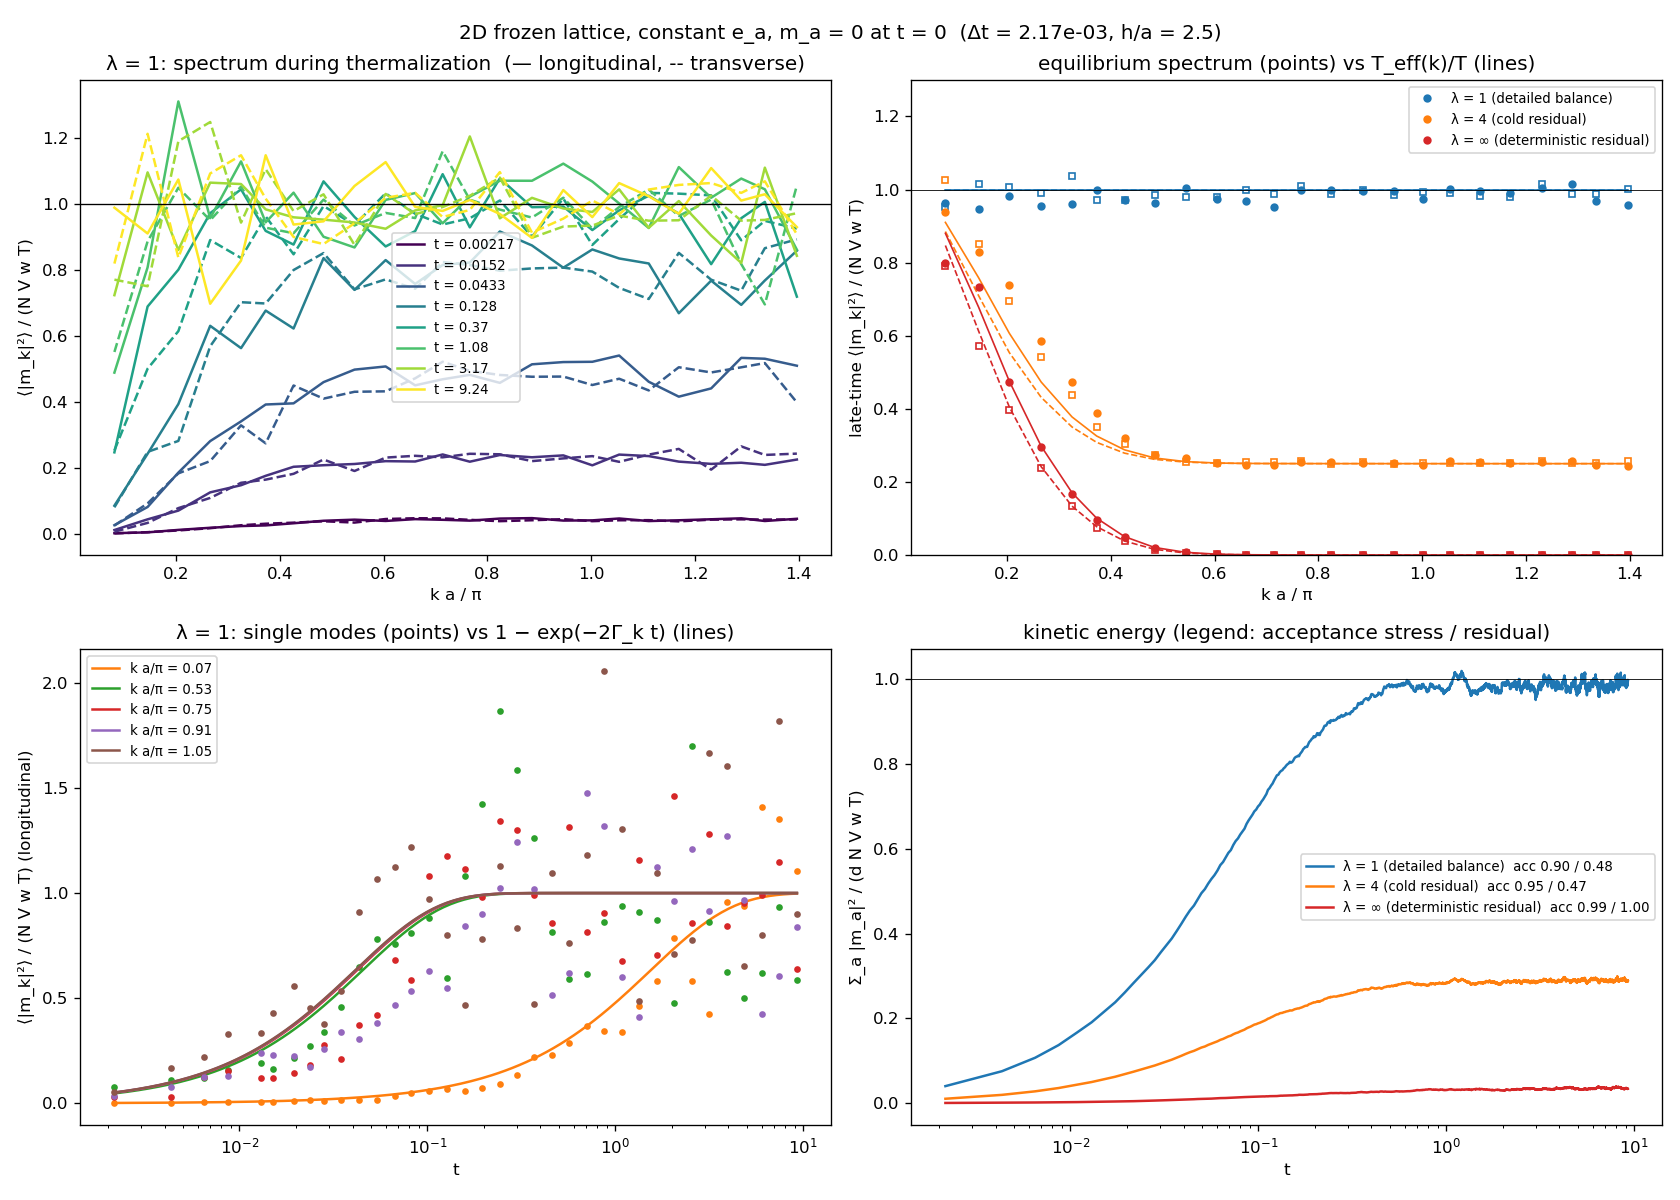
\includegraphics[width=\textwidth]{figs/stochrep_thermalize_2d.png}
\caption{As \Fig{fig:therm1d}, in 2D.  Solid lines and filled points:
longitudinal; dashed lines and open points: transverse.}
\label{fig:therm2d}
\end{figure}

\paragraph{Small $k$.}  \Fig{fig:smallk}: a 1D lattice of length 2 (160
particles), started from a thermal draw, 64 runs.  Every mode shown except
the lowest relaxes at least ten times during the run; the lowest only 2.5
times, and its error is large (a run eight times longer gives
$0.965\pm0.032$ there, against $0.995$).  For $\lambda=\infty$ the deficit
$1-T_{\rm eff}/T$ vanishes as $k^2$, and the measurement follows it.  Close to the
prediction there remains a small deficit that is a time-step error: relative to
$T_{\rm eff}$, at $ka/\pi=0.1$--$0.2$,
\begin{center}
\begin{tabular}{lcc}
$\Delta t$ / default & bond vote & single vote \\ \hline
$1/4$  & $-3\%$   & $-3\%$ \\
$1/16$ & $-1.5\%$ & $-0.5\%$
\end{tabular}
\end{center}
It does not depend on the vote, so it comes from the explicit residual step,
not from the rejections.

\begin{figure}[t]
\centering
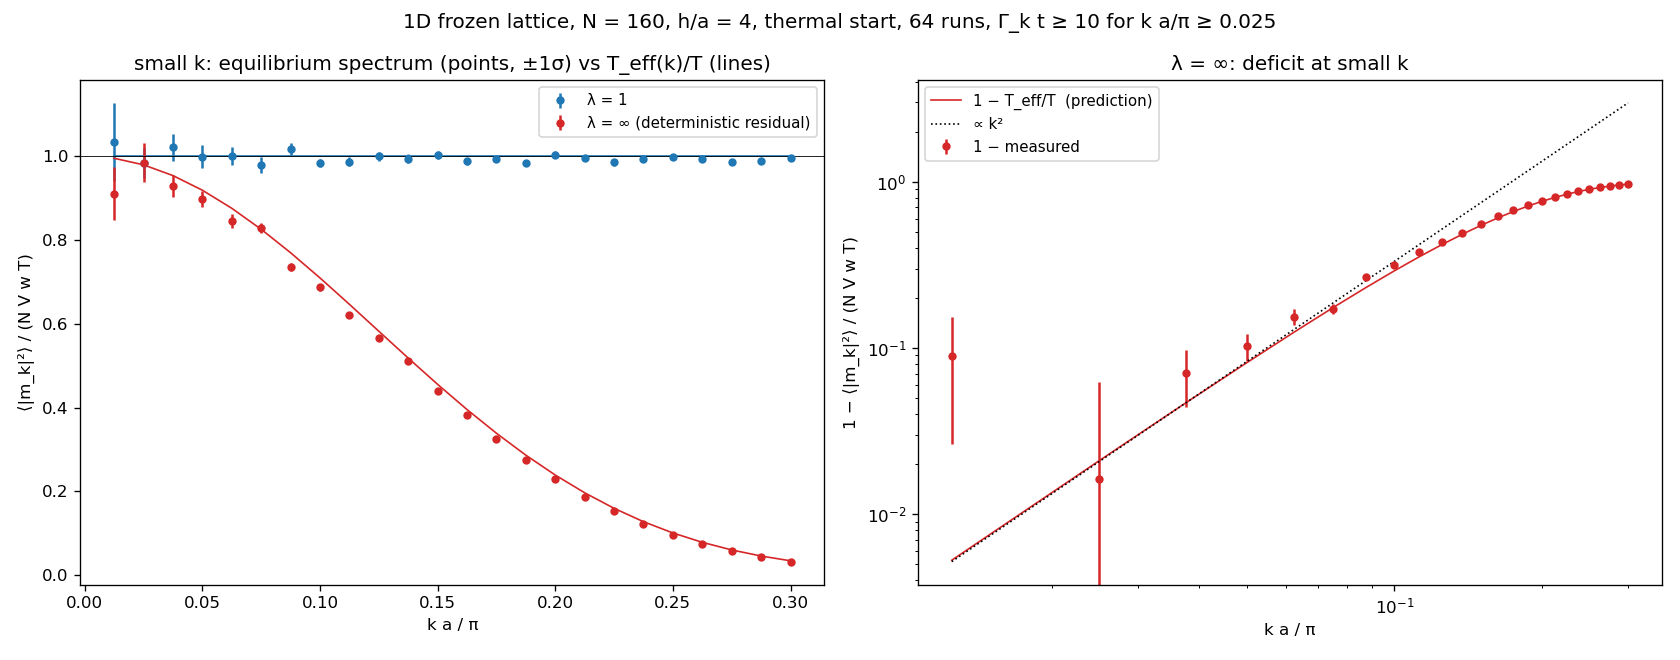
\includegraphics[width=\textwidth]{figs/stochrep_smallk.png}
\caption{1D, small $k$.  Left: the equilibrium spectrum ($\pm1\sigma$) for $\lambda=1$
and $\lambda=\infty$, with $T_{\rm eff}(k)/T$ (lines).  Right: the deficit
$1-\avg{|m_k|^2}/(NV_awT)$ for $\lambda=\infty$, and the prediction, $\propto k^2$.}
\label{fig:smallk}
\end{figure}

\paragraph{Acceptance.}  Rejections fall as $\sqrt{\Delta t}$.  The residual move,
with 88 bonds in 2D, is rejected most:
\begin{center}
\begin{tabular}{lccc}
residual move & bond vote, \Eq{sigmaab} & even split & single vote \\ \hline
1D, at rest            & 0.75 & 0.79 & 0.89 \\
1D, moving at $v=0.32$ & 0.73 & 0.18 & 0.89 \\
2D, at rest            & 0.48 & 0.58 & 0.88 \\
2D, moving at $v=0.32$ & 0.47 & 0.07 & 0.88
\end{tabular}
\end{center}
In 2D, at the full default step, the bond vote accepts 0.35 of the residual
moves and the single vote 0.77; at $1/16$ of it, 0.76 and 0.94.  These tables
were measured without the grid shift.

\paragraph{Still to do.}
\begin{enumerate}
\item The proposal coefficients are evaluated in the rest frame; they need
  the comoving forms of the deterministic step for a moving fluid.
\item \emph{Energy.}  Follow $H$ and the temperature over long runs.
\item \emph{Hydrodynamics.}  With the Hamiltonian step on: the equilibrium
  spectrum of a uniform fluid, and ensemble-averaged sound and shear decay.
\end{enumerate}

%=============================================================================
\section{Is the residual move needed?}
\label{sec:needresid}

With the stress move alone a mode is damped, and receives noise, only through
the fitted gradient, at the rate $R(k)\Gamma(k)$, where $R(k)=K_{\rm res}(k)/K(k)$ is the
fraction of the bond dissipation that the fit sees.  $R$ falls from one for
$kh\ll1$ to zero beyond $kh\simeq4$, so most lattice modes are invisible to the stress
move.  With the Hamiltonian step on, these modes are heated by the ideal SPH
force and run away unless the residual move damps them.  The runs that show
this, and the first long runs with the Hamiltonian step, are documented in
\texttt{fullruns.tex}.

%=============================================================================
\section{A moving fluid}
\label{sec:moving}

The construction carries over to a fluid moving with velocity $\bm v$, with
the same substitutions as in the deterministic bond form
(\texttt{bond\_dissipation.tex}, the moving fluid): bonds are measured in the
rest frame of the particle, the metric $\delta$ is replaced by the comoving
metric $\ell$, and the scalar part of the strain is removed along the projector
$P$.  The consensus, the partition of $\Delta S_a$ and the sweep are unchanged.

\paragraph{Ingredients.}  For particle $a$, with velocity $\bm v_a$,
$\gamma_a=1/\sqrt{1-v_a^2}$, temperature $T_a=\partial H/\partial s_a$ and rest-frame
temperature $(T_{\rm rel})_a=\gamma_aT_a$:
\begin{itemize}
\item the thermal vector is $\beta_a=\bm v_a/T_a=\gamma_a\bm v_a/(T_{\rm rel})_a$, and still
  \st
  \frac{\partial S_a}{\partial\bm m_a}\Big|_{e_a}=-\beta_a ;
  \stp
\item the comoving metric and the scalar projector,
  \st
  \ell^{ij}=\delta^{ij}-v^iv^j,\qquad
  P_{ij}=-c_s^2u_iu_j+\frac1d\big(\delta_{ij}+u_iu_j\big),\qquad
  \avg{P\ell}\equiv P_{ij}\ell^{ij}=1-c_s^2v^2 ,
  \stp
  with $u_i=\gamma v_i$;
\item bond weights evaluated at the rest-frame bond length, normalized so that
  the bond moment is the comoving metric,
  \st
  \sum_{b\neq a}w_{ab}\,\bm r_{ab}\bm r_{ab}^T=\ell_a ;
  \stp
\item the face covector
  \st
  A_{ab\,k}=V_a\,w_{ab}\,(\ell_a^{-1}\bm r_{ab})_k ,
  \qquad \sum_{b\neq a}A_{ab\,k}\,r^j_{ab}=V_a\,\delta_k{}^j ;
  \label{Amoving}
  \stp
\item the fit, now
  \st
  (\nabla\beta)_a=\sum_{b\neq a}w_{ab}\,\Delta\beta_{ab}\,\bm r_{ab}^T\,\ell_a^{-1},\qquad
  (\nabla_k\beta_i)_a=\sum_{b\neq a}\frac{1}{V_a}\,(\Delta\beta_{ab})_i\,A_{ab\,k} .
  \label{Gmoving}
  \stp
\end{itemize}
\paragraph{Which velocity.}  The comoving metric, the projector, the bond lengths
and $\kappa(\bm v)$ are coefficients of the coarse-grained flow.  They are evaluated
with the coarse-grained particle velocity
\st
\bm v_a\to\dot{\bm x}_a=\frac{\partial H}{\partial\bm m_a},
\stp
the velocity with which the particles move, which varies slowly.  The
particle's own velocity, from $(e_a,\bm m_a)$, fluctuates thermally and is not
used here; it enters only through $\beta_a$ in the entropy.  The coefficients
are frozen at the start of the step, so the proposals are fixed symmetric
Gaussians as before, and $e^{\mathbb S}$ is stationary whatever velocity is used;
the choice affects only the coefficients, at order $h^2$.

\paragraph{The stress move.}  The resolved part of the dissipative function is
\st
K_{{\rm res},a}=\frac12V_a\,(T_{\rm rel}\kappa^{ijmn})_a\,(\nabla_j\beta_i)_a(\nabla_n\beta_m)_a
=V_a\Big[(T_{\rm rel}\eta)_a\tr\big(\ell_a\mathring S_a\ell_a\mathring S_a\big)+\tfrac12(T_{\rm rel}\zeta)_a\theta_a^2\Big],
\stp
with $\mathring S=S-\theta P$, $S$ the symmetric part of $\nabla\beta$ and
$\theta=\ell^{ij}S_{ij}/\avg{P\ell}$.  Draw the stress with
\st
\avg{\xi_a^{ij}\xi_a^{mn}}=\frac{2\Delta t\,(T_{\rm rel})_a}{V_a}\,\kappa_a^{ijmn}(\bm v_a),
\stp
and distribute it through the faces,
\st
\mathsf p^i_{ab}=\xi_a^{ik}A_{ab\,k} .
\stp
By \Eq{Amoving} the virial is again the stress,
\st
\sum_{b\neq a}\mathsf p^i_{ab}\,r^j_{ab}=V_a\,\xi_a^{ij} ,
\stp
which is symmetric: no torque.  The linear entropy change is, by \Eq{Gmoving},
\st
\Delta\mathbb S=-\sum_{b\neq a}(\Delta\beta_{ab})_i\,\mathsf p^i_{ab}=-V_a\,\xi_a^{ik}(\nabla_k\beta_i)_a,
\stp
exactly as at rest, and the argument of \Sect{sec:stress} gives
\st
\avg{\xi_a^{ij}}=-\Delta t\,(T_{\rm rel})_a\,\kappa_a^{ijmn}(\nabla_n\beta_m)_a=\Delta t\,\Pi_a^{ij}(\nabla\beta),\qquad
\avg{\mathsf p^i_{ab}}=\Delta t\,\Pi_a^{ik}(\nabla\beta)\,A_{ab\,k} ,
\stp
the traction of the resolved part of the moving bond form.

\paragraph{Drawing the stress.}  Write the quadratic form in whitened
variables.  With $\hat e_1=(\hat x\hat x-\hat y\hat y)/\sqrt2$ and
$\hat e_2=(\hat x\hat y+\hat y\hat x)/\sqrt2$ an orthonormal basis of traceless
symmetric matrices, define
\st
E_k=\ell^{1/2}\hat e_k\,\ell^{1/2}-\frac{P_{ij}(\ell^{1/2}\hat e_k\ell^{1/2})^{ij}}{\avg{P\ell}}\,\ell ,
\qquad k=1,2 .
\stp
Then, with $z_1,z_2,z_3$ independent unit Gaussians,
\st
\xi_a=\sqrt{\frac{2\Delta t\,(T_{\rm rel})_a}{V_a}}\Big[\sqrt{2\eta_a}\,\big(z_1E_1+z_2E_2\big)
+\sqrt{\zeta_a}\,z_3\,\frac{\ell}{\avg{P\ell}}\Big]
\stp
has the covariance above.  At rest $E_k=\hat e_k$ and $\ell=\one$, and this is the
draw of \Sect{sec:stress}.  (With unresolved dimensions, $\zeta\to\zeta_{\rm eff}$.)

\paragraph{The residual move.}  The residual part is
\st
K_{{\rm resid},a}=(T_{\rm rel}\eta)_a\sum_{b\neq a}V_aw_{ab}\,\delta_{ab}(\beta)\cdot\ell_a\cdot\delta_{ab}(\beta),
\qquad \delta_{ab}\beta=\Delta\beta_{ab}-(\nabla\beta)_a\,\bm r_{ab} .
\stp
Draw on each bond
\st
\mathfrak p_{ab}=\sqrt{2\Delta t\,c_{ab}/\lambda}\;\ell_a^{1/2}\bm z_{ab},\qquad
c_{ab}=(2T_{\rm rel}\eta)_a\,V_aw_{ab},
\stp
with $\bm z_{ab}$ a vector of independent unit Gaussians, so
$\avg{\mathfrak p_{ab}\mathfrak p_{ab}^T}=2\Delta t\,c_{ab}\,\ell_a/\lambda$.  Remove the part
the fit sees, now through the face covector $A_{ab\,k}$ of \Eq{Amoving}: the
bond index $k$ of the virial of the draws is contracted with it,
\st
\vec p^{\,i}_{ab}=\mathfrak p^i_{ab}-\frac1{V_a}\Big(\sum_{c\neq a}\mathfrak p^i_{ac}\,r^k_{ac}\Big)A_{ab\,k} .
\stp
By \Eq{Amoving}, $\sum_bA_{ab\,k}\,r^j_{ab}=V_a\,\delta_k{}^j$, its virial vanishes,
$\sum_b\vec p^{\,i}_{ab}r^j_{ab}=\sum_c\mathfrak p^i_{ac}r^j_{ac}-\sum_c\mathfrak p^i_{ac}r^j_{ac}=0$.
The linear entropy change is $-\sum_b\mathfrak p_{ab}\cdot\delta_{ab}\beta$, and since the
residuals are still orthogonal to the bonds (the orthogonality involves no
metric), the mean of the virial of the draws vanishes and
\st
\avg{\vec p^{\,i}_{ab}}=-\Delta t\cdot(2T_{\rm rel}\eta)_a\,V_aw_{ab}\,\ell_a^{ij}(\delta_{ab}\beta)_j ,
\stp
the residual part of the moving bond traction.  The two moves together give
the deterministic traction $-(2T_{\rm rel}\eta)_a\,V_aw_{ab}\,\ell_a\,\mathcal D_{ab}\beta$ on
every bond, plus the mean-field force of the bulk and dilation terms, as at rest.

\paragraph{The consensus.}  Unchanged.  The bond factor is still, to leading
order, $-(\beta_b-\beta_a)\cdot\pf_{ab}$, so it is not affected by the
background flow; this is why the partition \Eq{sigmaab} was chosen
(\Sect{sec:tests}: in a fluid moving at $v=0.32$ the acceptance is the same as
at rest).

\paragraph{The equilibrium.}  The stationary distribution is still
$e^{\mathbb S}$ at fixed $e_a$.  Around a moving state the momentum fluctuations
are no longer isotropic.  To quadratic order their covariance per particle is
the inverse of minus the Hessian of $S_a$ at fixed $e_a$,
\st
\avg{\delta m^i\,\delta m^j}=V_a\,\Big[\big(\chi^{-1}\big)_{ij}\Big]^{-1},\qquad
\chi^{-1}_{\mu\nu}=\frac{\partial\beta_\mu}{\partial T^{0\nu}} ,
\label{Cmoving}
\stp
the spatial block of the inverse susceptibility of \texttt{theory.tex},
inverted.  It is not the spatial block of $\chi$ itself: holding $e_a$ fixed
conditions on the energy.  From \texttt{theory.tex},
\st
\chi^{-1}_{ij}=\frac{1}{(e+p)\gamma\,T_{\rm rel}}\Big[\frac{4c_s^2}{1-c_s^2v^2}\,u_iu_j+\delta_{ij}+u_iu_j\Big].
\stp
For $v=0.5$ along $x$ and $c_s^2=1/3$ this gives $C_{xx}=0.733\,V_awT$ along the flow
and $C_{yy}=1.333\,V_awT$ across it; a numerical Hessian of $S_a$ agrees to four
digits.

Beyond quadratic order, the single-particle distribution in a large system at
fixed total momentum is $e^{S_a(e_a,\bm m_0+\delta\bm m)+\bm\lambda\cdot\delta\bm m}$, with the
multiplier $\bm\lambda$ of the total momentum chosen so that $\avg{\delta\bm m}=0$
($\bm\lambda\simeq\beta_0$; setting it equal to $\beta_0$ shifts the mean by $0.09\sigma$
along the flow and the covariance by 1.7\%).  At $s_a=346$ its covariance is
$C_{xx}=0.722\,V_awT$ and $C_{yy}=1.316\,V_awT$, within 1.5\% of \Eq{Cmoving}.

\paragraph{Test.}  \Fig{fig:moving}: the 2D frozen hexagonal lattice of
\Sect{sec:tests}, moving at $v=0.5$ along $x$ (and at rest, for comparison),
stochastic step only, $\lambda=1$, starting from $\delta\bm m=0$.  Eight runs.
\begin{itemize}
\item The stress noise reproduces $\kappa^{ijmn}(\bm v)$ of the code to machine
  precision, at $v=0$, $0.58$ and $0.79$, with and without bulk viscosity.
\item The late-time spectrum, normalized by the exact covariance, is flat in
  $k$ for both polarizations.  Averaged over particles, $\avg{\delta m_x^2}/C_{xx}=0.996$
  and $\avg{\delta m_y^2}/C_{yy}=0.999$ at $v=0.5$; a separate run from a thermal
  start gives $\avg{\delta m_x^2}/C_{xx}=1.000\pm0.002$, with either vote.
\item The acceptance is the same as at rest, and the total momentum is
  conserved to $10^{-14}$.
\end{itemize}

\begin{figure}[t]
\centering
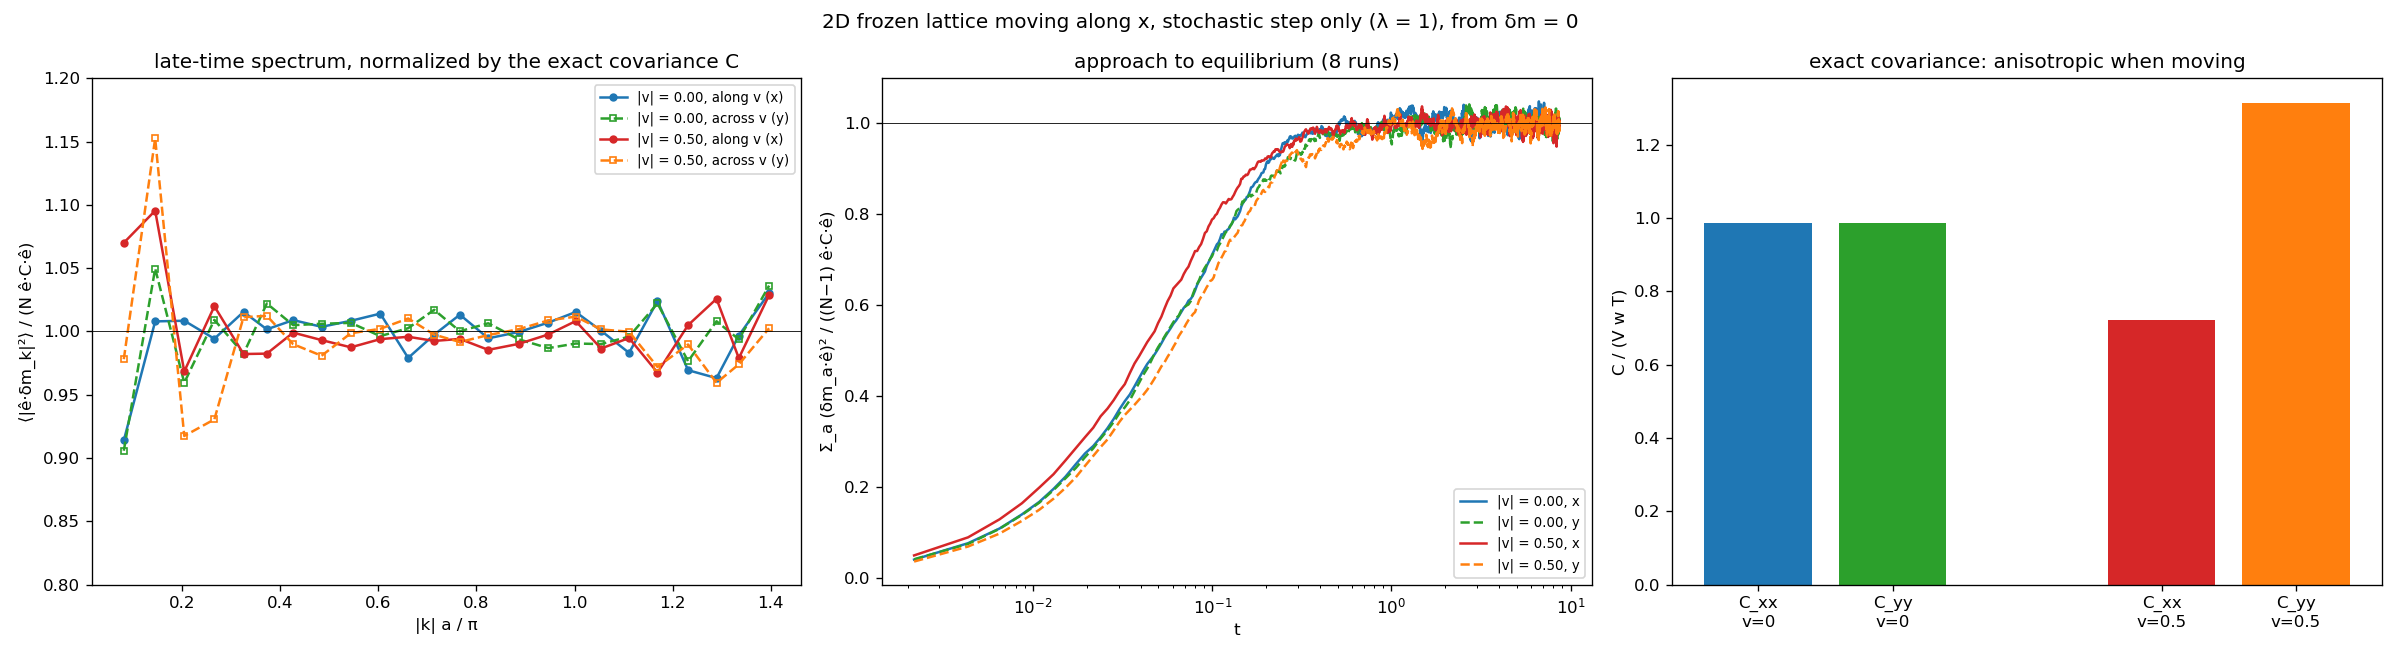
\includegraphics[width=\textwidth]{figs/stochrep_moving.png}
\caption{2D frozen lattice moving along $x$ at $v=0.5$, and at rest; stochastic
step only, $\lambda=1$, from $\delta\bm m=0$.  Left: late-time spectrum of the momentum
fluctuations along and across the flow, normalized by the exact covariance.
Middle: approach to equilibrium.  Right: the exact covariance, anisotropic when
the lattice moves.}
\label{fig:moving}
\end{figure}

\paragraph{Implementation.}  In 2D the code uses the comoving forms above:
comoving weights and $\ell$ for each star, the face covector \Eq{Amoving} in both
moves, and the draws above.  The velocity is $\dot{\bm x}_a$ (\texttt{pa.dotx}),
in the stochastic step and in the deterministic bond force alike, so that the
mean of the one equals the other.  The coefficients use
$(T_{\rm rel})_a=\gamma_a\,\partial H/\partial s_a$; in the code \texttt{pa.T} is
$\partial H/\partial s_a=(T_{\rm rel})_a/\gamma_a$.  In 1D the rest-frame forms are used.

\end{document}
